\documentclass[a4paper, 12pt]{article}

\usepackage{cmap}
\usepackage{mathtext} 
\usepackage[T2A]{fontenc}
\usepackage[utf8]{inputenc}
\usepackage[english,russian]{babel}

\usepackage{amsfonts,amssymb,amsthm,mathtools}
\usepackage{amsmath}
\usepackage{icomma} 

\usepackage{graphicx} 
\graphicspath{{Picturies/}}
\usepackage{wrapfig}

\usepackage{array,tabularx,tabulary,booktabs}
\usepackage{longtable}
\usepackage{multirow}

\usepackage{caption}
\usepackage{subcaption}
\captionsetup{labelsep=period}

\renewcommand{\phi}{\varphi}
\newcommand{\eps}{\varepsilon}
\renewcommand{\AA}{\ensuremath{\mathring{A}}}
\newcommand{\parag}[1]{\paragraph*{#1:}}

\newcounter{Points}
\setcounter{Points}{1}
\newcommand{\point}{\arabic{Points}. \addtocounter{Points}{1}}

\author{Вязовцев Андрей, Б01-005}
\date{13.05.22}
\title{Лабораторная работа 4.3.3. Исследование разрешающей способности микроскопа методом Аббе.}

\begin {document}

\maketitle

\parag {Цель работы} изучение дифракционного предела разрешения объектива микроскопа.

\parag {В работе используются} лазер; кассета с набором сеток разного периода; линзы; щель с микрометрическим винтом; оптический стол c набором рейтеров и крепёжных винтов; экран; линейка.

\parag {Теоретическая справка} ~\\

Формула для расчета периодов решёток:
\begin{equation*}
	d \sin \phi = m \lambda
\end{equation*}

Формула для расчета увеличения микроскопа:
\begin{equation*}
	Г = \dfrac{b_1 b_2}{a_1 a_2}            
\end{equation*}

Формула для расчета минимального расстояния, разрешимого микроскопом:
\begin{equation*}
	d \geq \dfrac{\lambda}{\left( D / 2f \right)} 
\end{equation*}

\parag {Экспериментальная установка} ~

Схему рабочего места можно посмотреть на рис. \ref{pic1}.

\begin{figure}[!h]
    \centering
    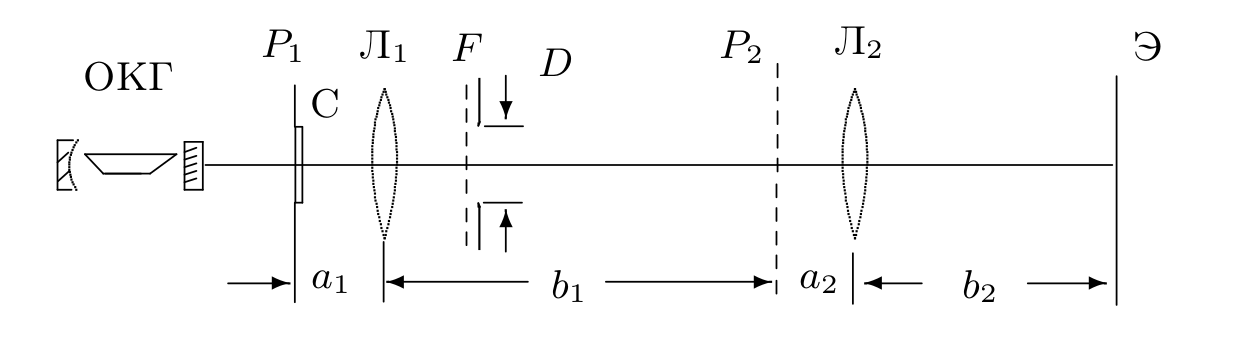
\includegraphics[scale = 0.3]{pic1.png}
    \caption{Модель проекционного микроскопа}
    \label{pic1}
\end{figure}

\parag {Ход работы} ~\\

\point Подготовим установку к работе, выпишем её основные характеристики: $L = 120 \pm 0.01$ см, $\lambda = 532 \pm 1$ нм.

\point Закрепим кассету с решетками, пронаблюдаем дифракционные картины для разных сеток. Измерим расстояния между соседними дифракционными максимумами для каждой решетки.

\begin{table}[!h]
	\centering
\begin{tabular}{|c|c|c|c|c|c|} \hline
	№ решетки & 1 & 2 & 3 & 4 & 5 \\ \hline
	Расстояние, мм & 31.3 & 21.0 & 10.5 & 5.2 & 4.3 \\ \hline
\end{tabular}
\end{table}

\point Соберем модель проекционного микроскопа. Запишем его характеристики: $F_1 = 110$ мм, $F_2 = 25$ мм,  $a_1 = 64 \pm 1$ мм, $a_2 = 280 \pm 1$ мм, $b_1 = 500 \pm 1$ мм, $b_2 = 380 \pm 1$ мм. Посчитаем увеличение микроскопа $Г \approx 10.6 \pm 0.3$. Измерим периоды изображений сеток на экране:

\begin{table}[!h]
	\centering
\begin{tabular}{|c|c|c|c|c|c|} \hline
	№ решётки & 1 & 2 & 3 & 4 & 5 \\ \hline
	b, мм & 30 & 50 & 50 & 133 & 146 \\ \hline
	n & 14 & 14 & 8 & 10 & 8 \\ \hline
	Период, мм & 2.1 & 3.6 & 6.3 & 13.3 & 18.3 \\ \hline
\end{tabular}
\end{table}

\point Поместим щелевую диафрагму с микрометрическим винтом в фокальную плоскость $F$ линзы $Л_1$ . Определим для каждой решётки минимальный размер диафрагмы, при котором на экране еще видно изображение сетки (при меньших размерах щели изображение выглядит как одномерная решётка).

\begin{table}[!h]
	\centering
\begin{tabular}{|c|c|c|c|c|} \hline
	№ решетки & 1 и 2 & 3 & 4 & 5 \\ \hline
	D, мм & Не видно & 1.64 & 1.22 & 1.05 \\ \hline
\end{tabular}
\end{table}

\point Проведём качественный опыт по пространственной фильтрации. Для этого будет поворачивать щель и наблюдать максимумы по разным направлениям. Результаты занесём в таблицу:

\begin{table}[!h]
	\centering
\begin{tabular}{|c|c|c|c|} \hline
	положение & n, ед. & l, мм & период, мм \\ \hline
	вертикальное   & 15 & 100 & 6.7 \\ \hline % не копипаста, само так вышло. А вообще, зачем я это мерил?
	горизонтальное & 15 & 100 & 6.7 \\ \hline
	диагональное   & 15 & 100 & 6.7 \\ \hline
\end{tabular}
\end{table}

\point Получим мультиплицированное изображение для всех сеток. Для этого изменим установку по методичке. При этом установим ширину щели $D = 0.16$ мм. Заметим, что при сужении щели изображения уменьшаются, а при смене сетки уменьшается количество щелей.

\parag {Обработка результатов} ~\\

\point По измерениям спектра определим дифракционные углы и рассчитаем периоды решеток.

\begin{table}[!h]
	\centering
\begin{tabular}{|c|c|c|c|c|c|} \hline
	№ решетки & 1 & 2 & 3 & 4 & 5 \\ \hline
	$\phi$, $10^{-3}$ &  26.1 & 17.5 & 8.75 & 4.31 & 3.61 \\ \hline
	Период, мкм & 20 & 30 & 61 & 124 & 147 \\ \hline
\end{tabular}
\end{table}

% \point По измерениям увеличенных с помощью микроскопа изображений найдём периоды сеток:

% \begin{table}[!h]
% 	\centering
% \begin{tabular}{|c|c|c|c|c|c|} \hline
% 	Номер решетки & 1 & 2 & 3 & 4 & 5\\ \hline
% 	Период, мкм & 20 & 34 & 59 & 125 & 173 \\ \hline
% \end{tabular}
% \end{table}

% Хуй знает, как это считать и что нужно делать.

\point По измерениям с щелью рассчитаем период решетки:

\begin{table}[!h]
\centering
\begin{tabular}{|c|c|c|c|} \hline
	Номер решетки & 3 & 4 & 5 \\ \hline
	Период решетки, мкм & 16 & 22 & 25 \\ \hline
\end{tabular}
\end{table}

Измерения здесь, очевидно, не сошлись с предыдущими. К сожалению, автор не смог обнаружить ошибку в вычислениях.

% Ссанина, а не лабы.

\point Для проверки теории Аббе построим график зависимости $d = f \left( 1 / D \right)$. Периоды решеток возьмем определенные по спектру.

\begin{figure}[!h]
	\centering
	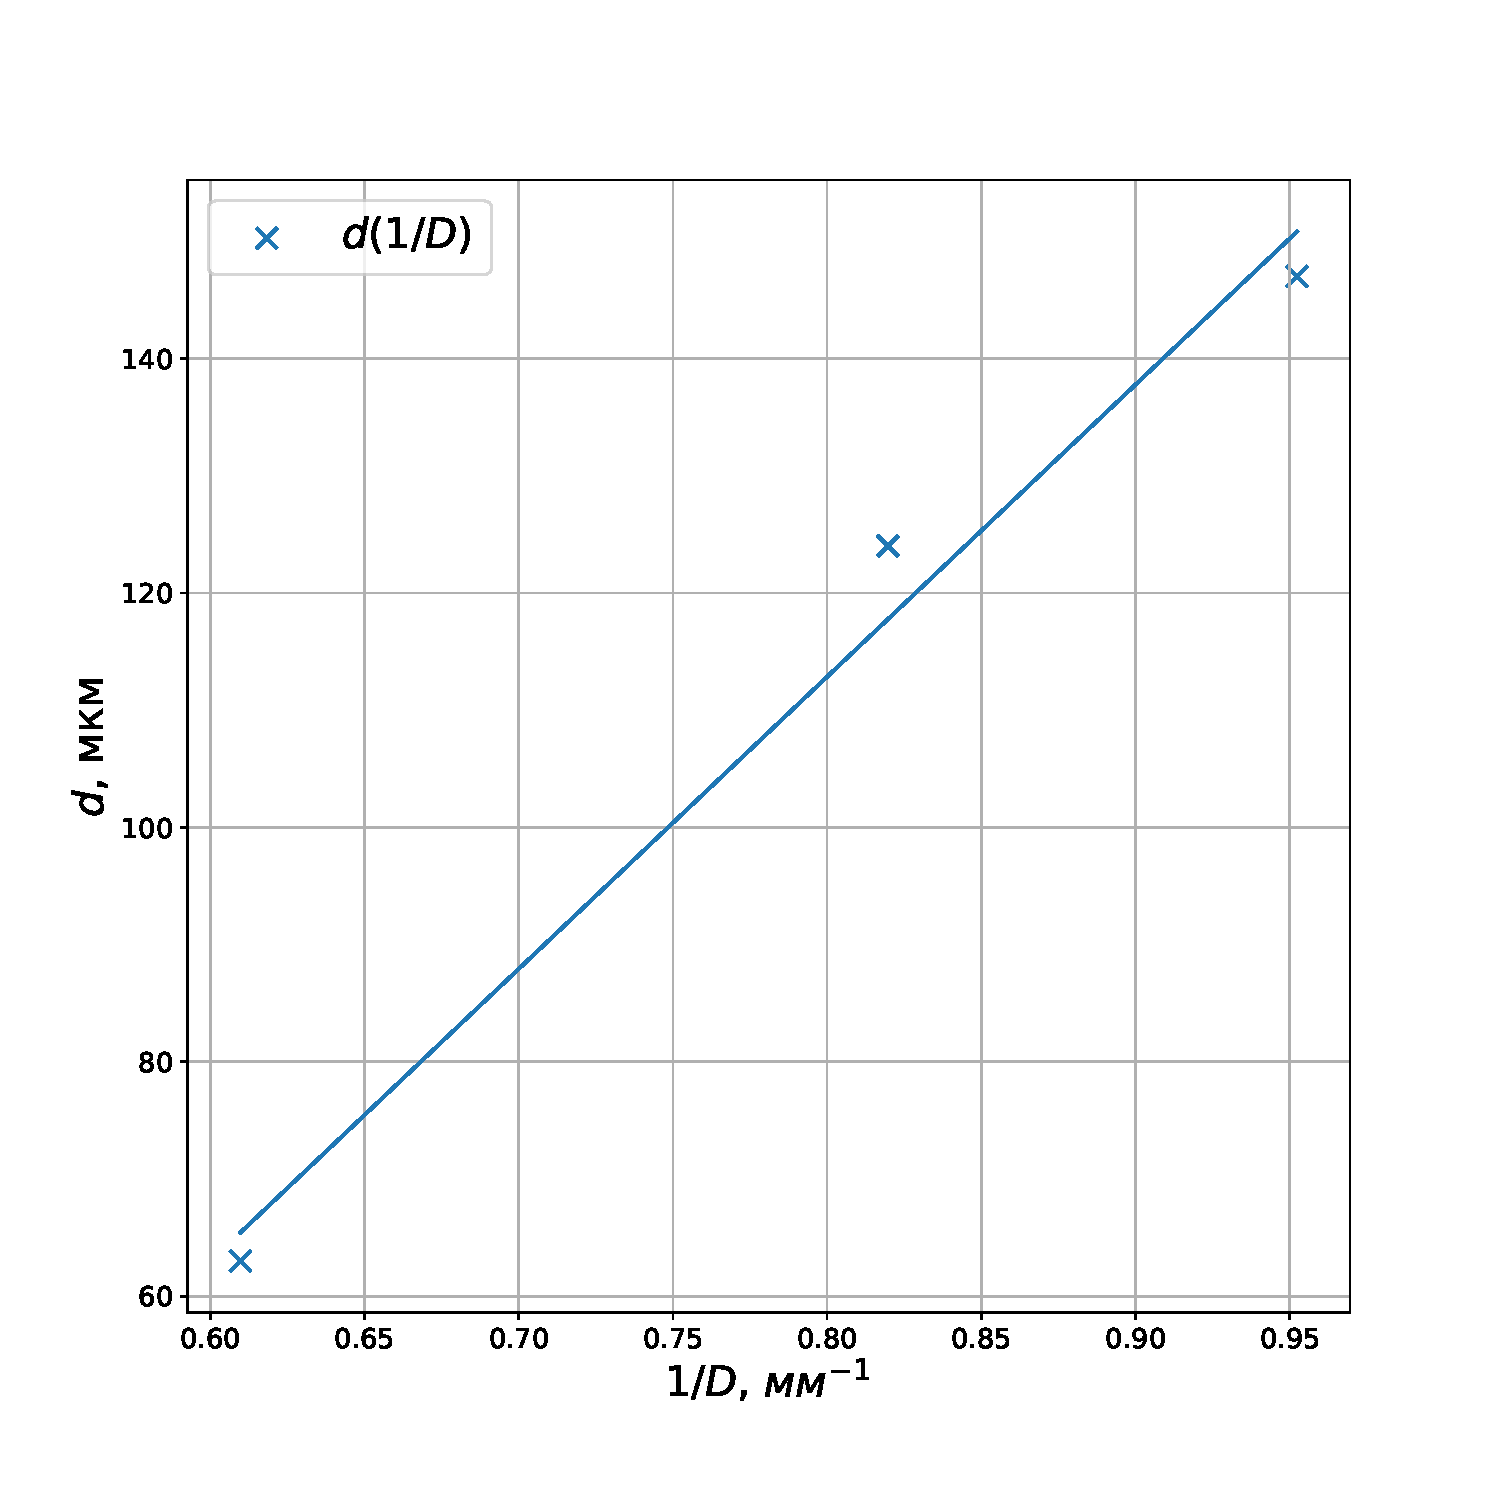
\includegraphics[scale = 0.4]{graph1}
	\caption{График зависимости $d = f \left( 1 / D \right)$}
	\label{graph1}
\end{figure}

\end {document}
